\documentclass{article}

\usepackage[utf8]{inputenc}
% \usepackage[english,greek]{babel}
\usepackage[unicode]{hyperref}
\usepackage[LGR, T1]{fontenc}
\usepackage{amsfonts, alphabeta, amssymb}
\usepackage[none]{hyphenat}
\usepackage{amsmath, slashed, graphicx, physics, tikz, braket, caption, subfig, comment, geometry, multicol, lipsum, fancyhdr, tcolorbox, siunitx, authblk, xcolor, abstract, float, indentfirst, xfrac, cancel, bbold, appendix, tikz, tikz-feynman, tensor, multirow, makecell, algpseudocode, algorithmicx, algorithm, changepage, adjustbox, lscape, placeins, xcolor, listings}
% \usepackage[style=numeric-comp,sorting=none]{biblatex}
% \setcounter{secnumdepth}{3}
% \setcounter{tocdepth}{3}
\title{
        \textbf{Study of a new kinematic weighting algorithm for the measurement of CP asymmetries in charm decays}
        \\
        LHCb Collaboration
}
\author{Georgios Christou}
\date{
        $4^{th}$ Week
        \\
        03/06/2023 - 07/07/2023
}

\lstset{language=C++,
        basicstyle=\ttfamily\small,
        keywordstyle=\color{blue},
        stringstyle=\color{red},
        commentstyle=\color{green!70!black},
        morecomment=[l][\color{magenta}]{\#},
        numbers=left,
        numberstyle=\tiny\color{gray},
        breaklines=true,
        frame=tb,
        columns=fullflexible,
        showstringspaces=false
}

\begin{document}
    \begin{figure}[t]
        \centering
        \subfloat{
\includegraphics[height = 3.5cm]{../../.images/CERN_logo.png}}
        \hspace{1cm}
        \subfloat{
\includegraphics[height = 3.5cm]{../../.images/Lhcb-logo-new.svg.png}}
    \end{figure}
    % \thispagestyle{empty}
    \maketitle

    \pagebreak
    
    \section{Introduction}

    We introduce a new TBranch to the TTree which includes randomly distributed values for the soft $\pi$ charge.

    \begin{lstlisting}
        TRandom3* random = new TRandom3();
        random->SetSeed();

        auto dataFramesPi = dataFrame.Define(
                "sPi_C", [random](){
                    return (random->Uniform() < 0.5) ? -1 : 1;
                }
        );
    \end{lstlisting}

    \begin{figure}[h!]
        \centering
        \subfloat{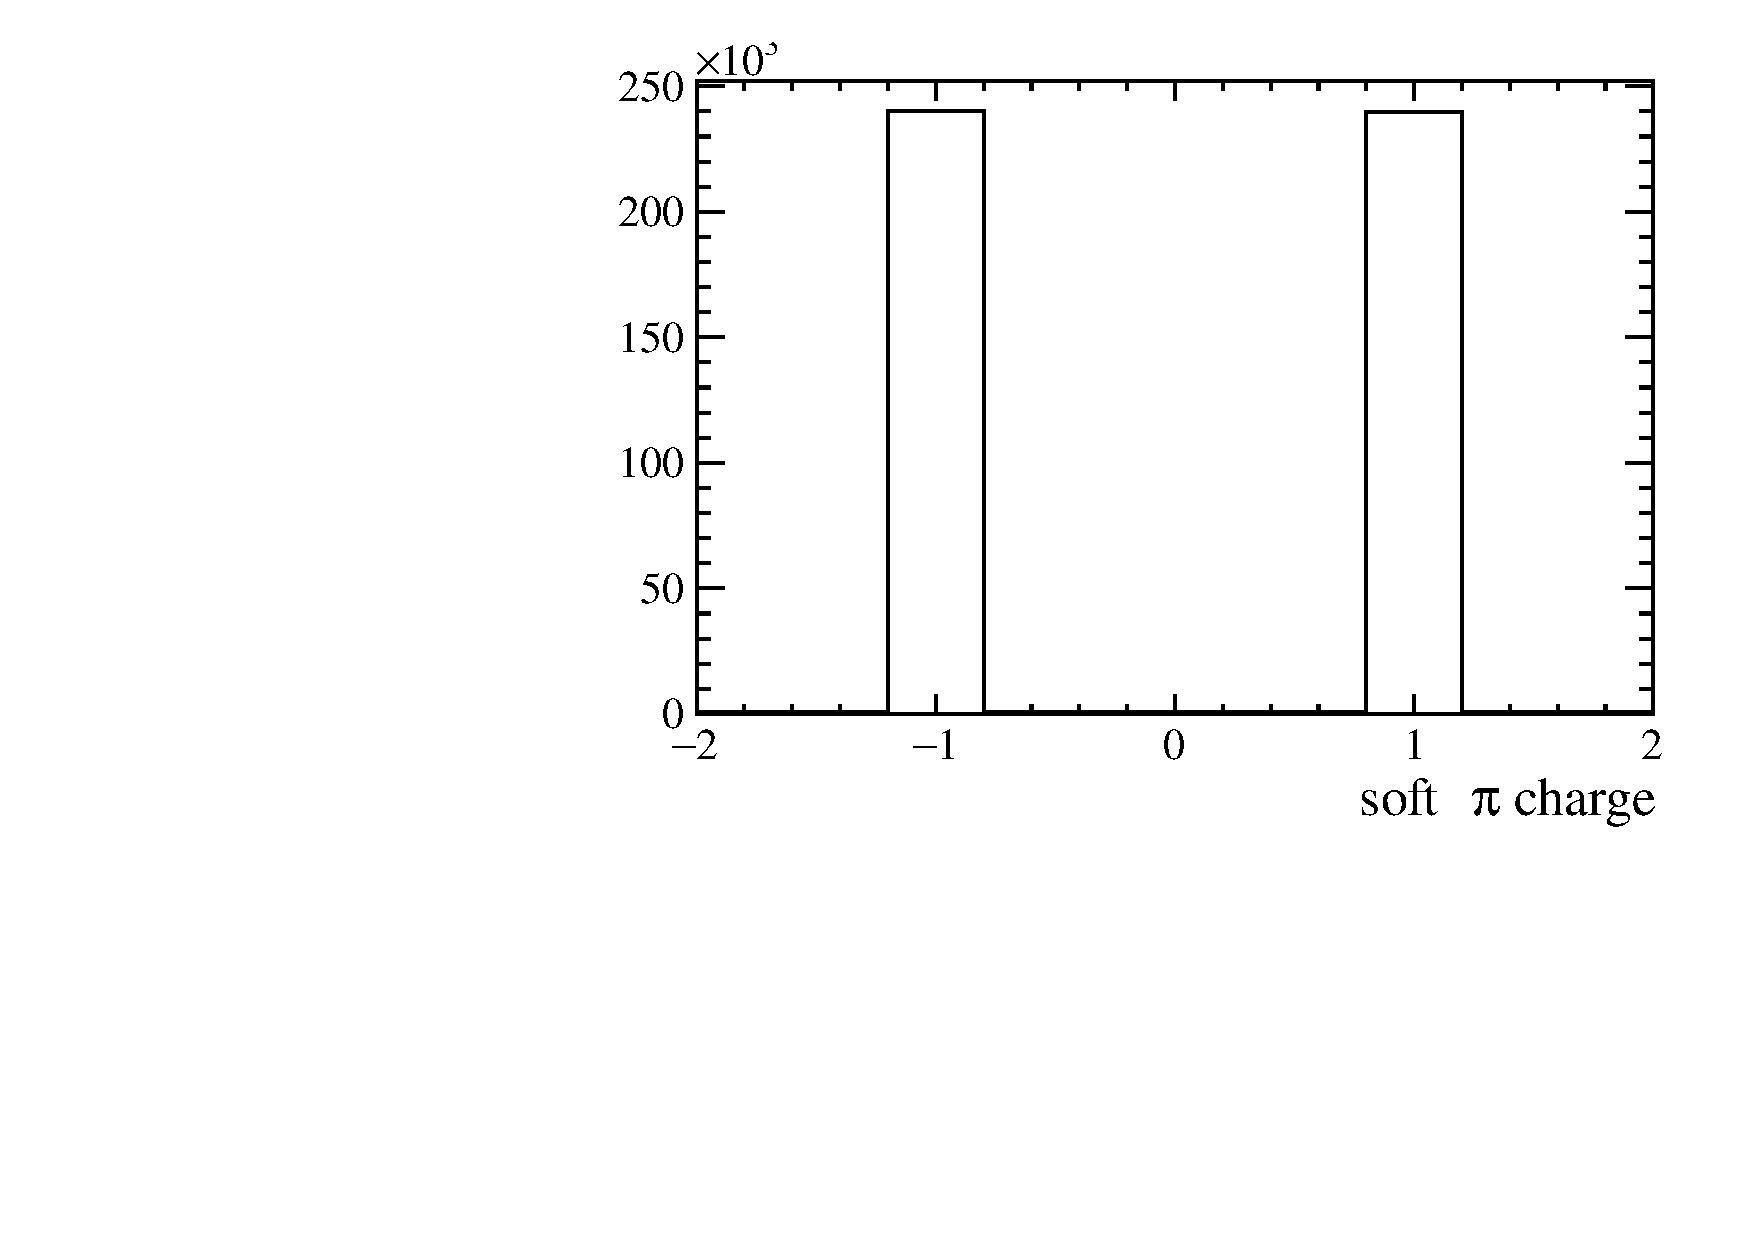
\includegraphics[width = 0.5\textwidth]{../../work/RapidSimAnalysis/MomentumDependence/Plots/sPi_C_KmKpInitial.pdf}}
        \subfloat{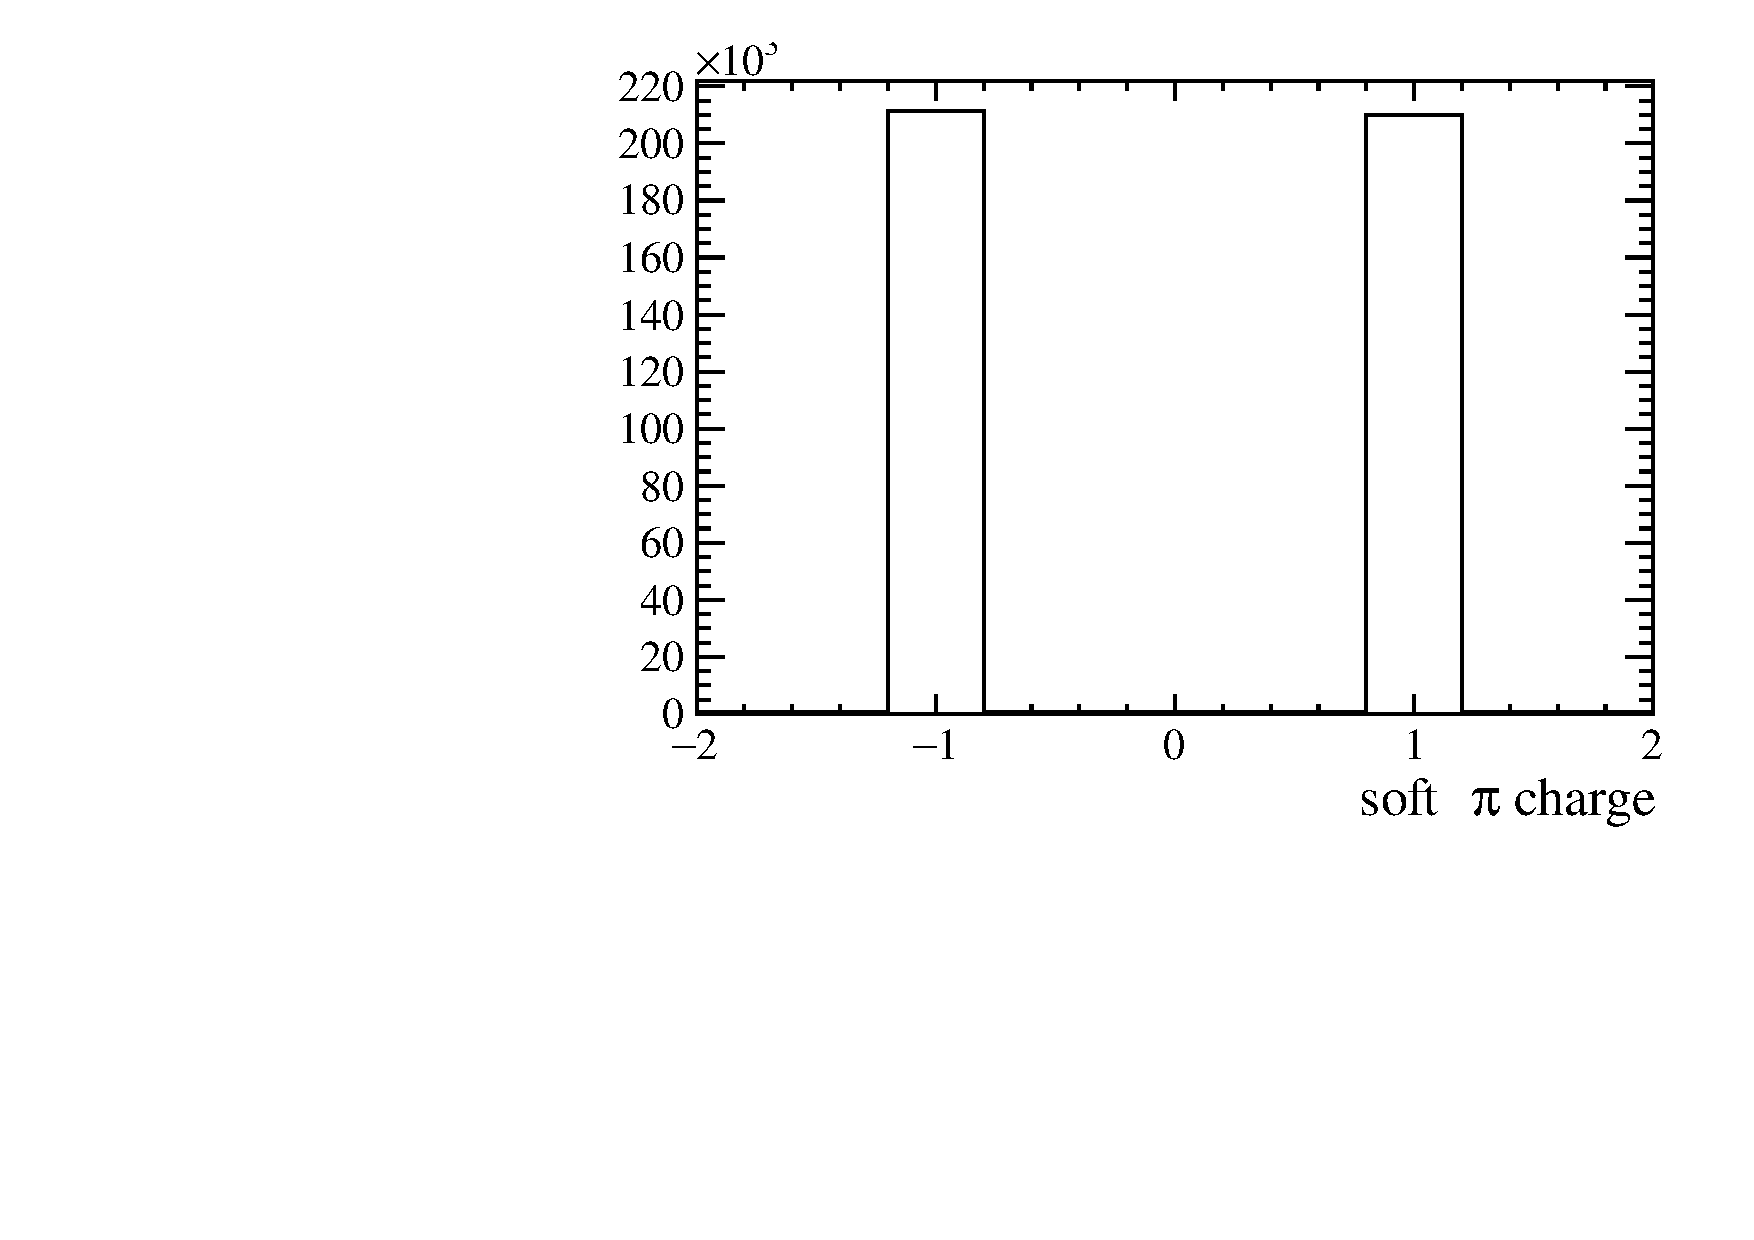
\includegraphics[width = 0.5\textwidth]{../../work/RapidSimAnalysis/MomentumDependence/Plots/sPi_C_pimpipInitial.pdf}}
        \caption{Initial soft $\pi$ charge distributions for $D^{0}\to K^-K^+$(left) and $D^{0}\to \pi^-\pi^+$(right).}
    \end{figure}

    Subsequently, $CP$ and detection asymmetries are introduced to filter out events and to emulate what we observe at LHCb.
    For the $CP$ asymmetry we keep all $\pi^+$ events and we filter out $\pi^-$ events according to the following probability:
    \begin{equation}
        P(\pi^-) = 1 - \frac{1 - A_{CP}}{1 + A_{CP}}
    \end{equation}

    \begin{lstlisting}
        auto dataFrameCP = dataFramesPi.Filter(
                [random, asymmetry](const int& sPi_C){
                        double probability;
                        probability = 1.0 - (1.0 - asymmetry)/(1.0 + asymmetry);

                        if (sPi_C == -1 && random->Uniform() < probability){
                                return false;
                        }
                        return true;
                }, {"sPi_C"}
        );
    \end{lstlisting}

    \begin{figure}[h!]
        \centering
        \subfloat{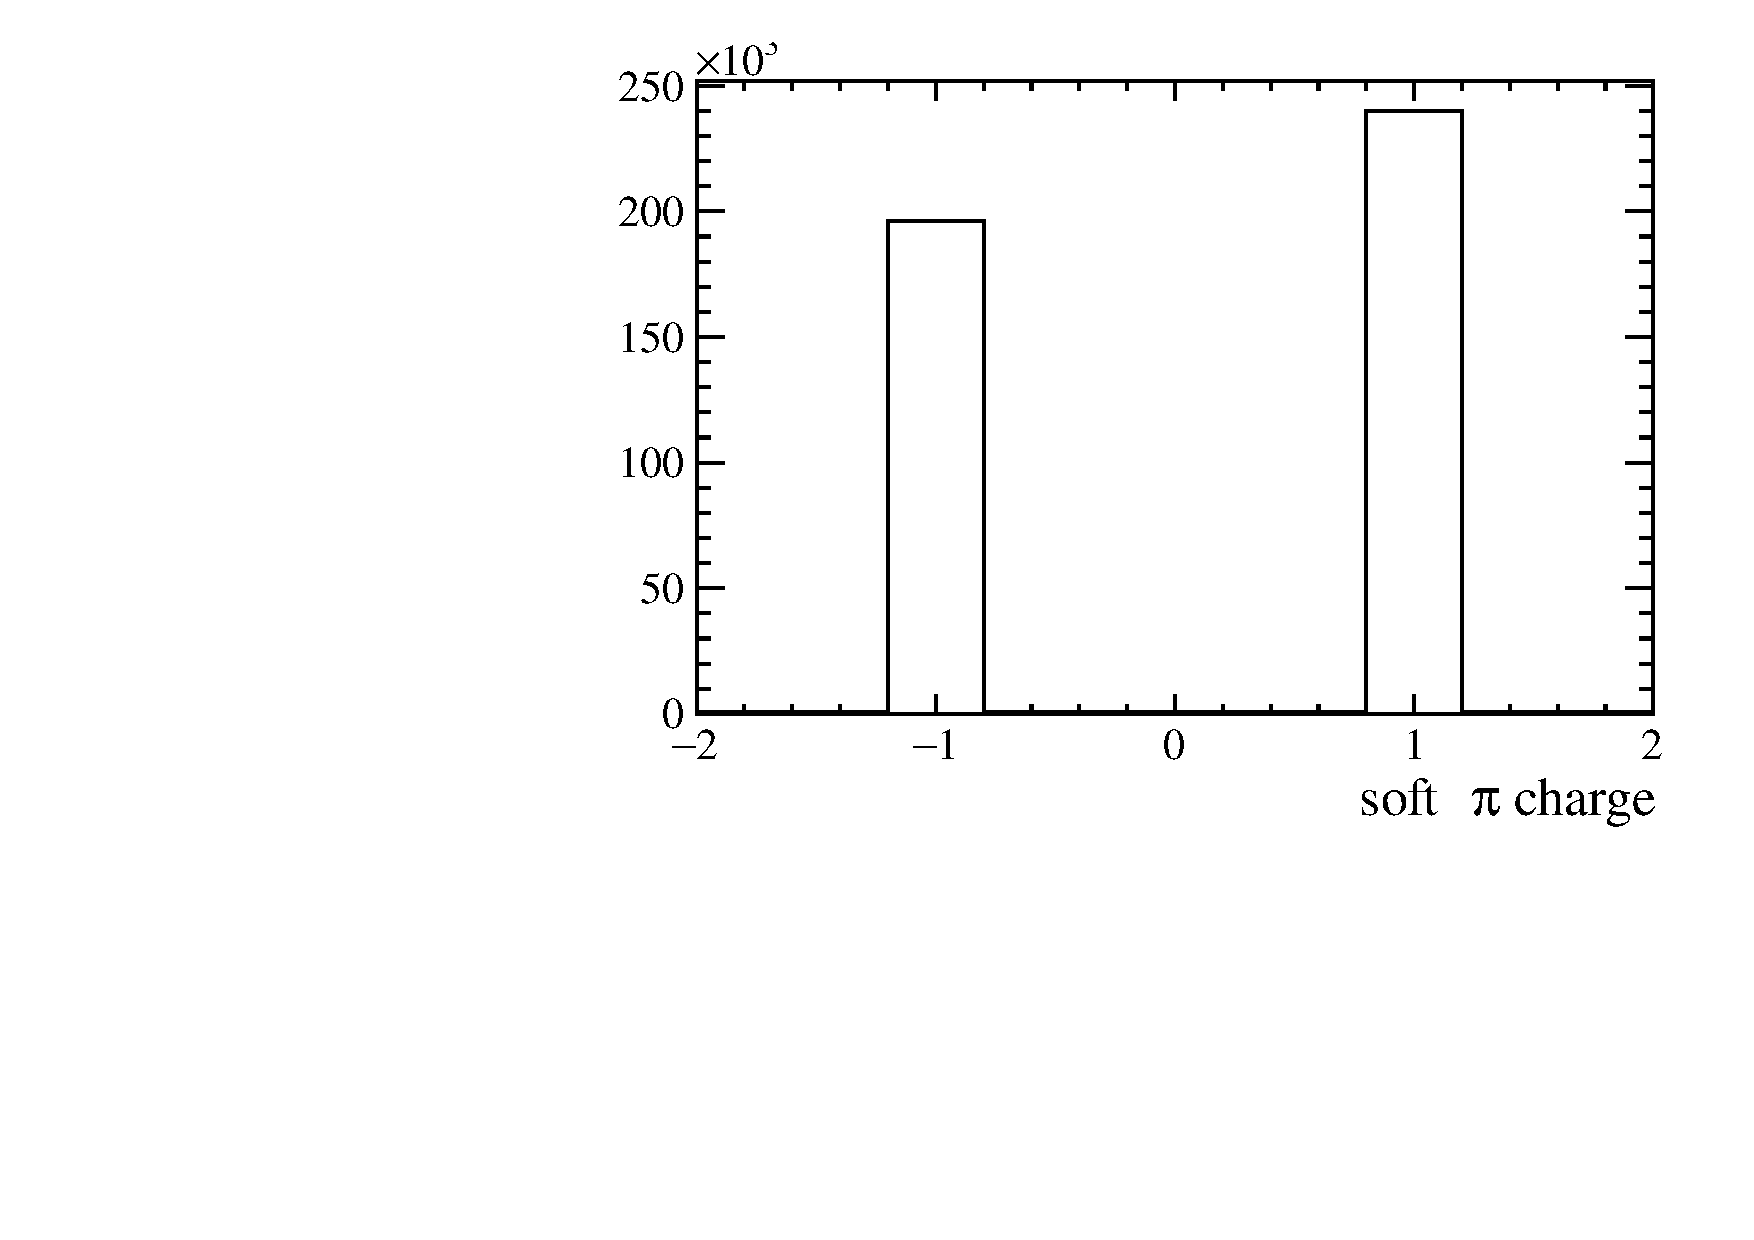
\includegraphics[width = 0.5\textwidth]{../../work/RapidSimAnalysis/MomentumDependence/Plots/sPi_C_KmKpCP.pdf}}
        \subfloat{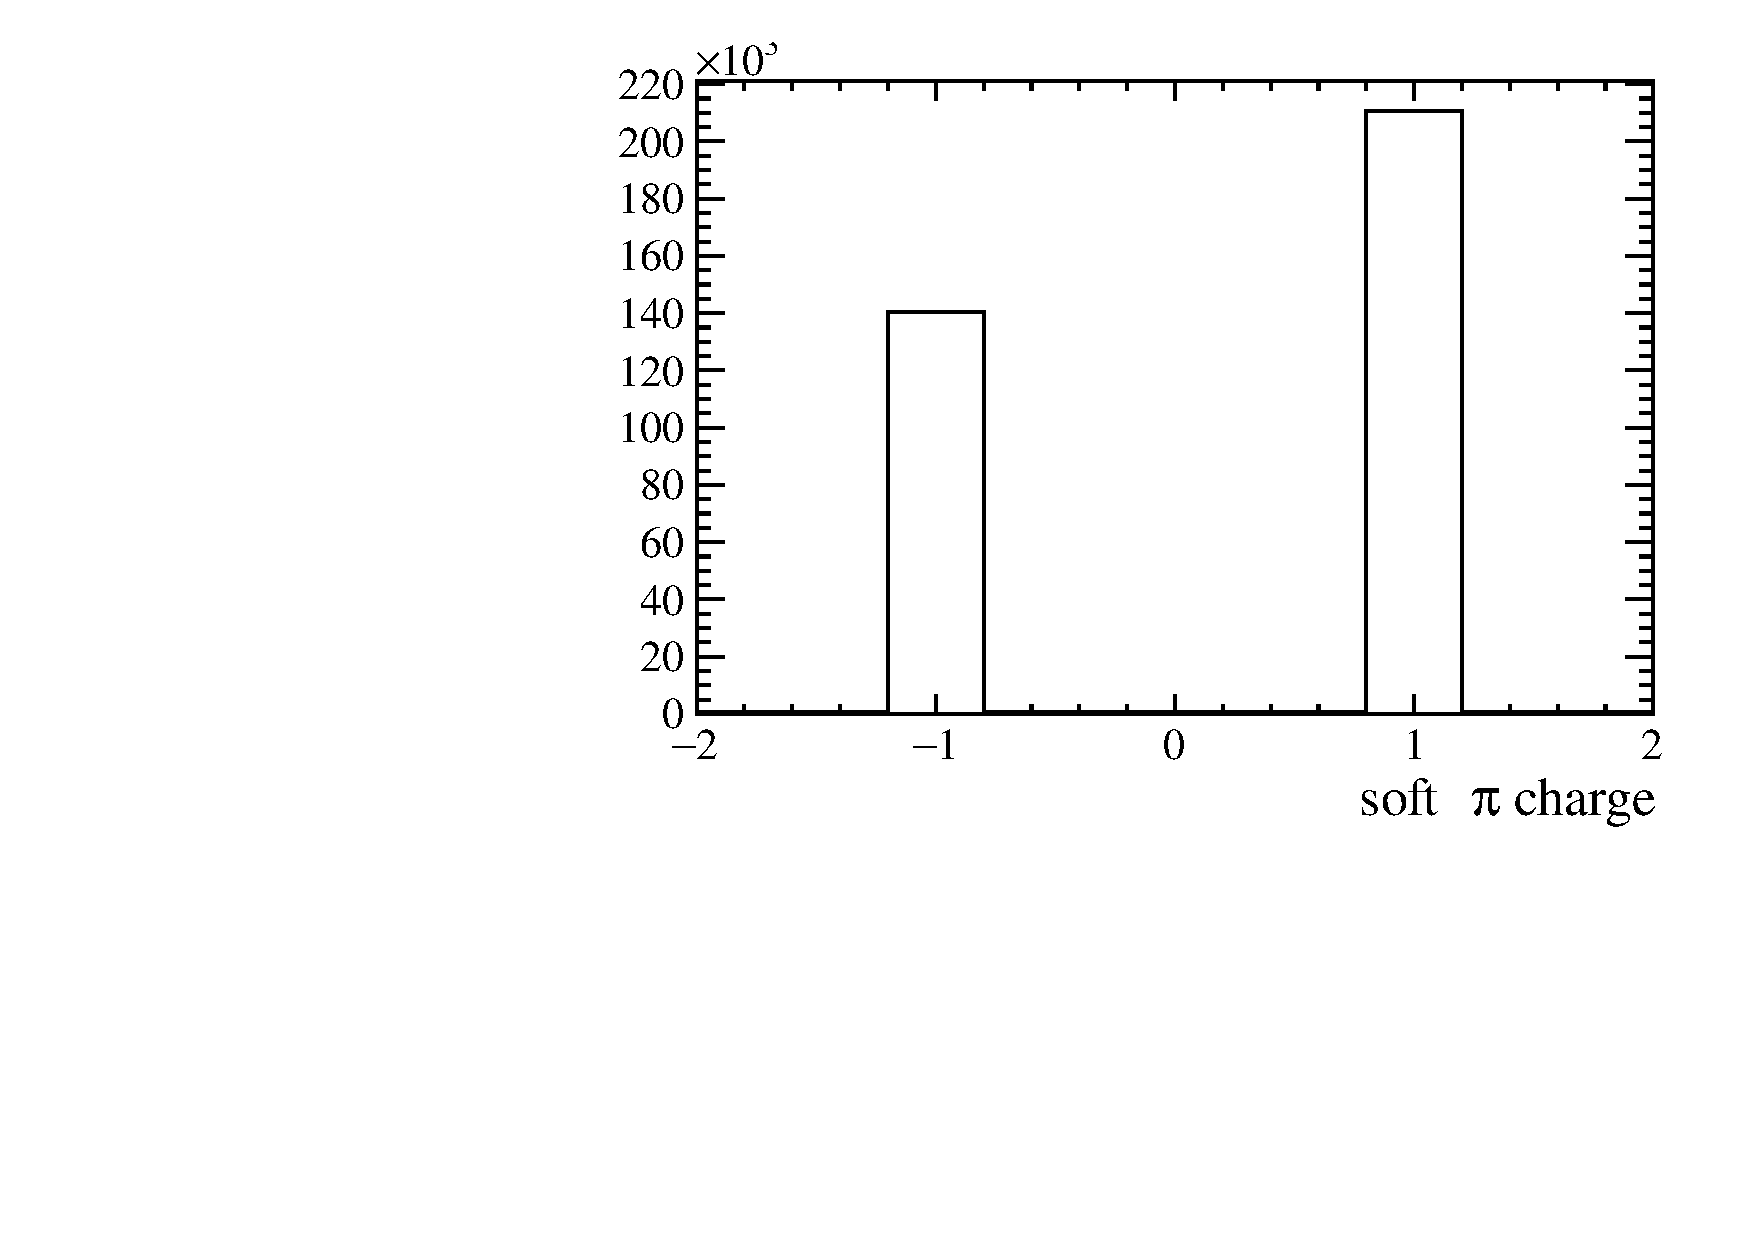
\includegraphics[width = 0.5\textwidth]{../../work/RapidSimAnalysis/MomentumDependence/Plots/sPi_C_pimpipCP.pdf}}
        \caption{Soft $\pi$ charge distributions for $D^{0}\to K^-K^+$(left) and $D^{0}\to \pi^-\pi^+$(right) after inrtoducing a $CP$ asymmetry.}
    \end{figure}


    Following the $CP$ asymmetry, we begin to inject a detection asymmetry with kinematic dependence.
    Namely, we define a line in the $p_x - p_z$ plane and filter out events according to the $p_x$ value of the soft $\pi$.

    \begin{lstlisting}
        double slope = 0.1;
        auto dataFrameDetection = dataFrameCP.Filter([slope](int& sPi_C, double& sPi_PX, double& sPi_PZ){
                if (sPi_C == -1 && (std::abs(sPi_PX) > slope*sPi_PZ)){
                        return false;
                }
                return true;
                }, {"sPi_C", "sPi_PX", "sPi_PZ"}
        );
    \end{lstlisting}
    \begin{figure}[h!]
        \centering
        \subfloat{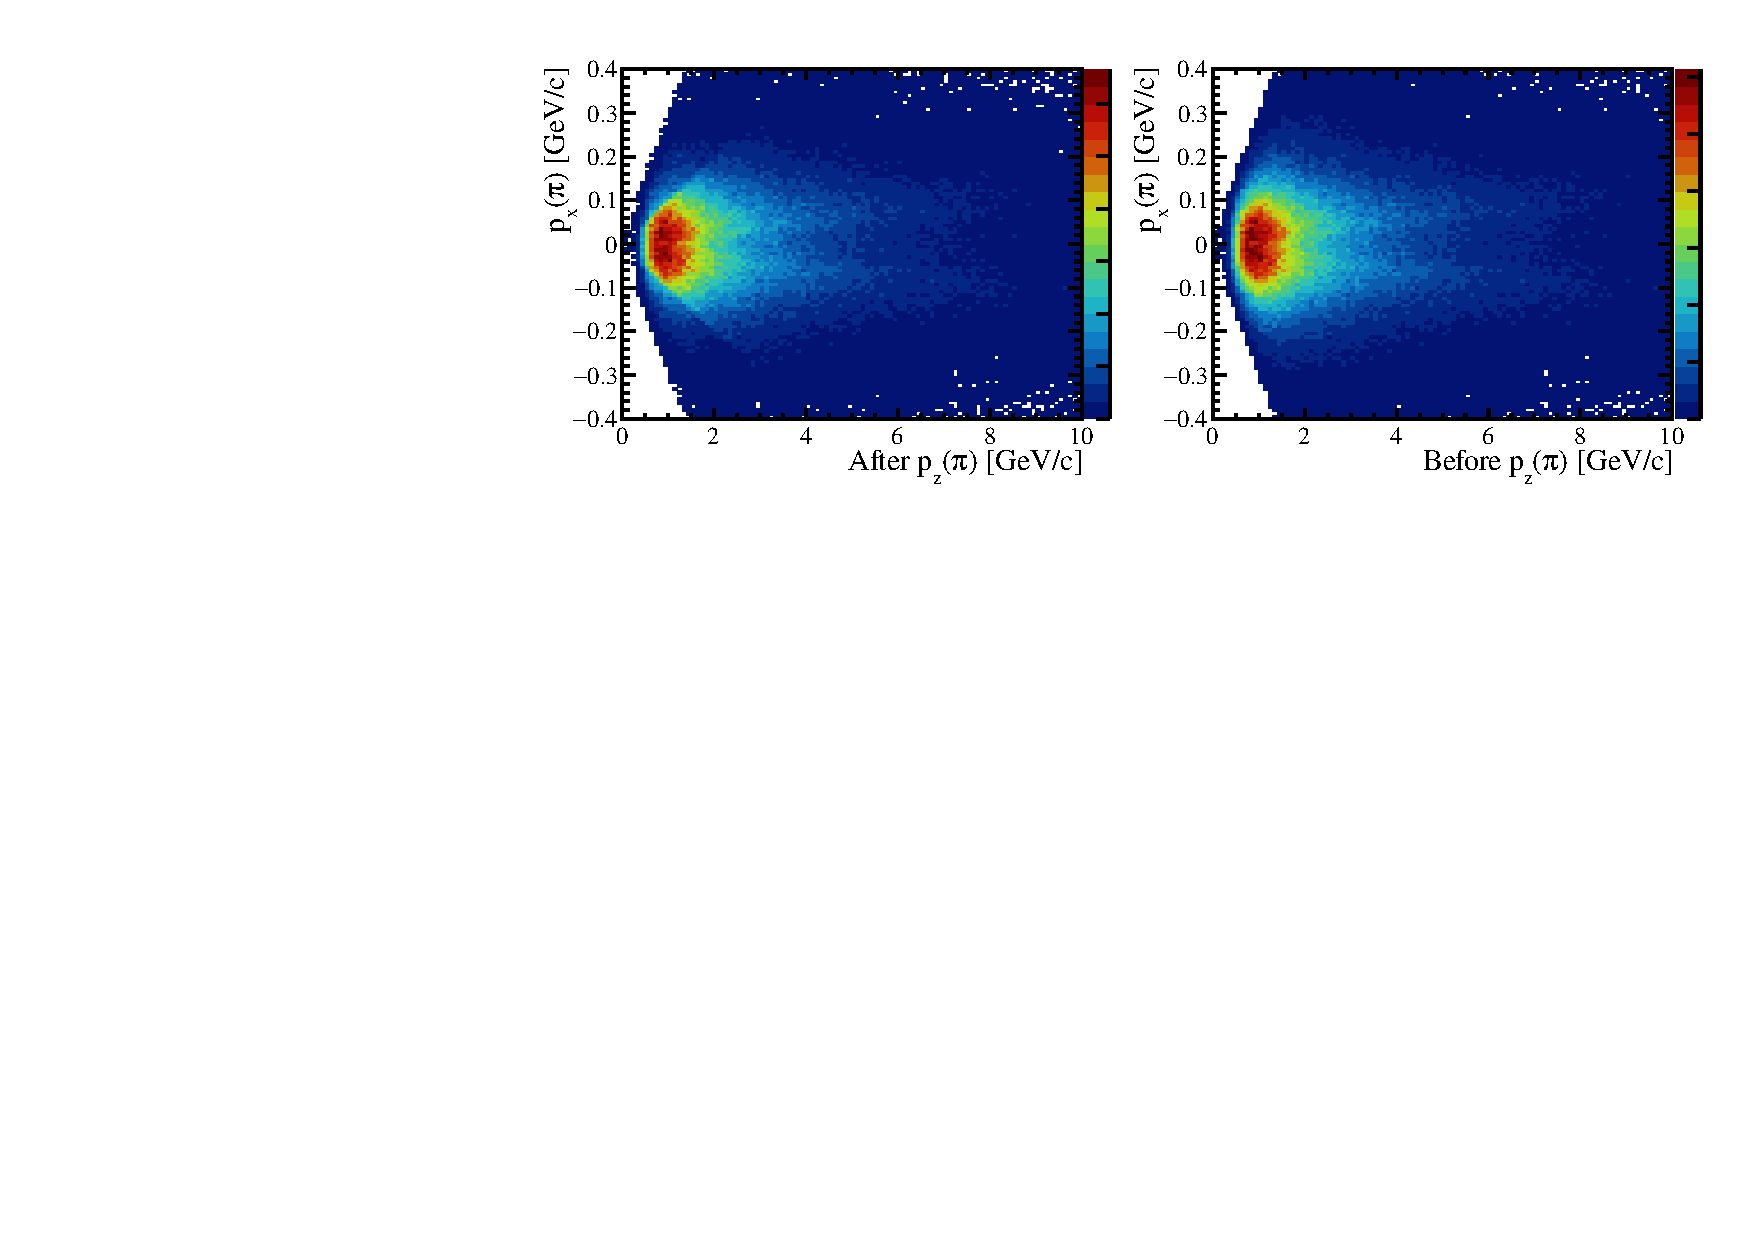
\includegraphics[width = \textwidth]{../../work/RapidSimAnalysis/MomentumDependence/Plots/sPi_C_KmKpBeforeAfter.pdf}}
        \hfill
        \subfloat{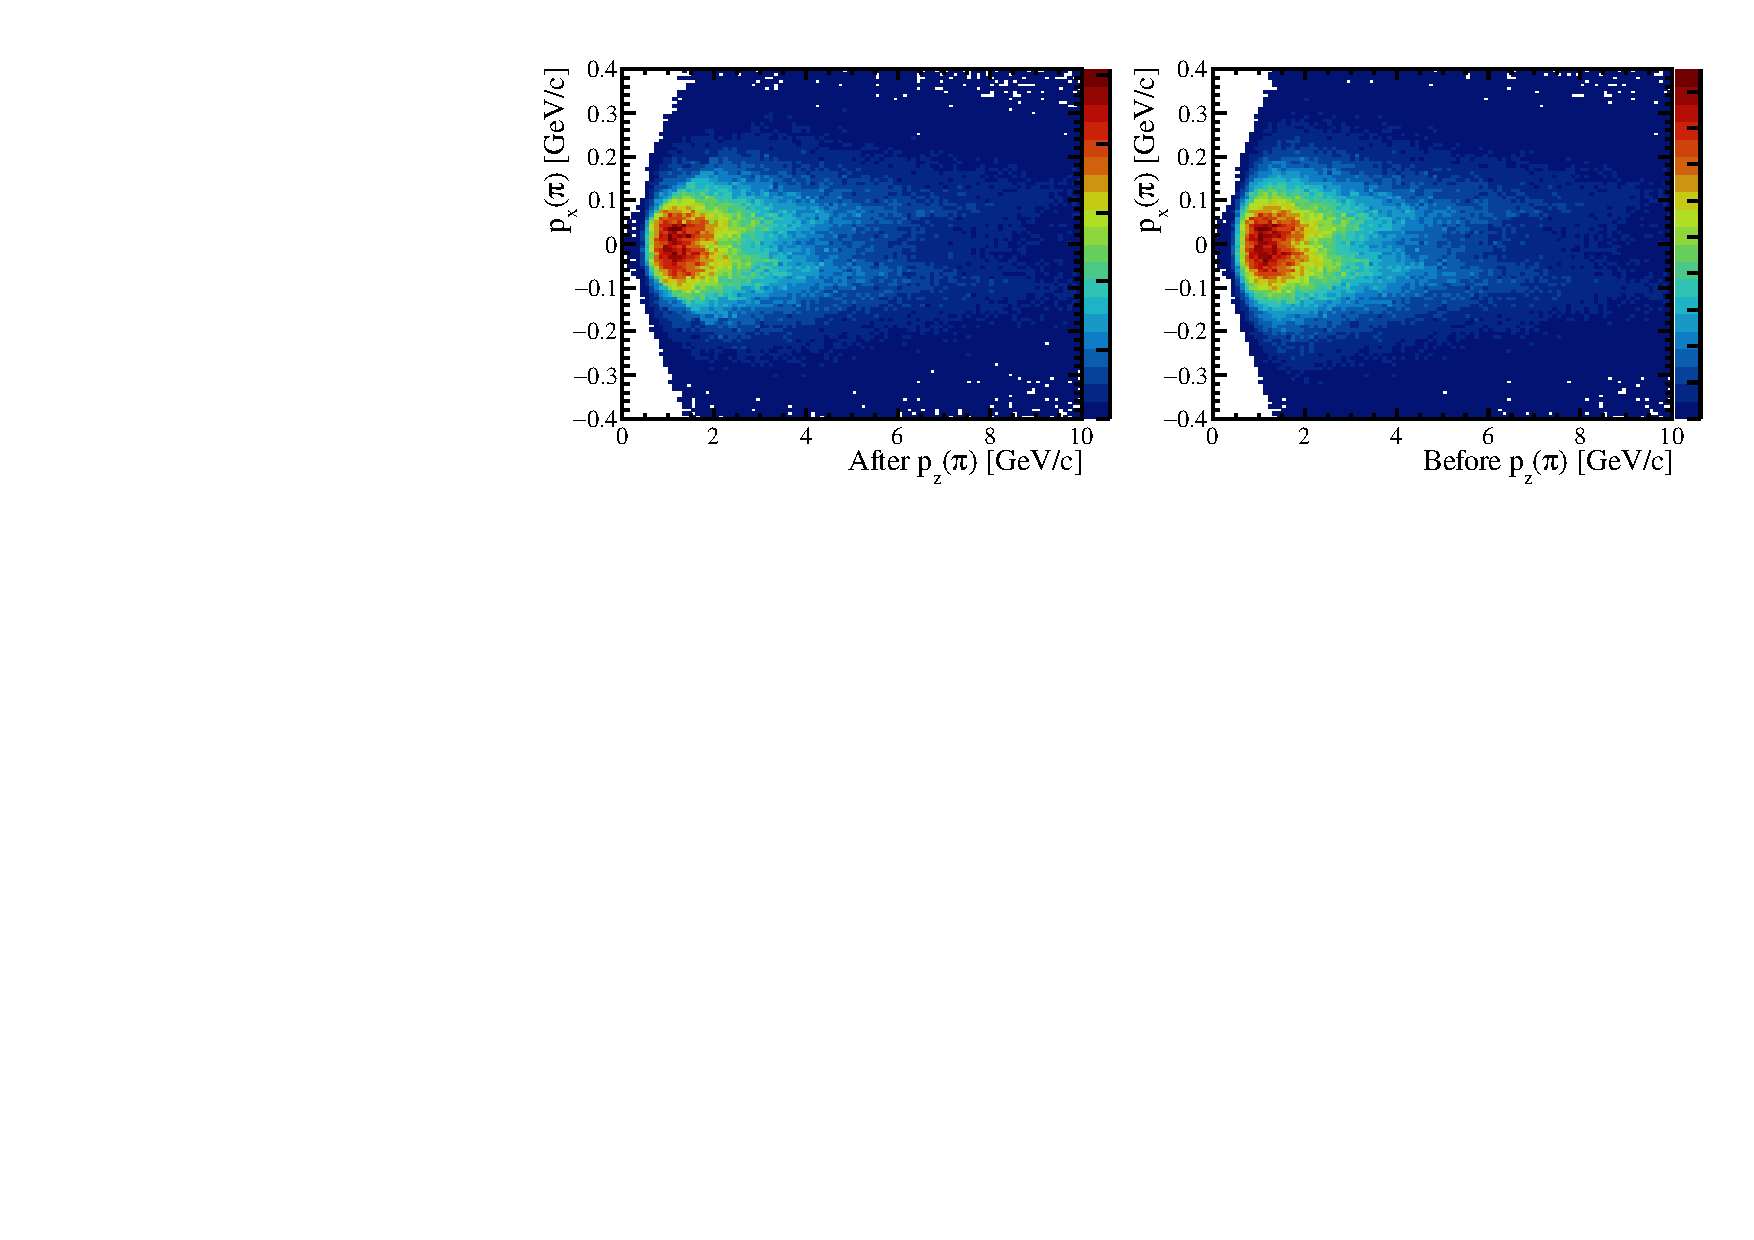
\includegraphics[width = \textwidth]{../../work/RapidSimAnalysis/MomentumDependence/Plots/sPi_C_pimpipBeforeAfter.pdf}}
        \caption{Soft $\pi$ $p_x - p_z$ plane for $D^{0}\to K^-K^+$(top) and $D^{0}\to \pi^-\pi^+$(bottom) before and after inrtoducing detection asymmetry.}
    \end{figure}

    \begin{figure}[h!]
        \centering
        \subfloat{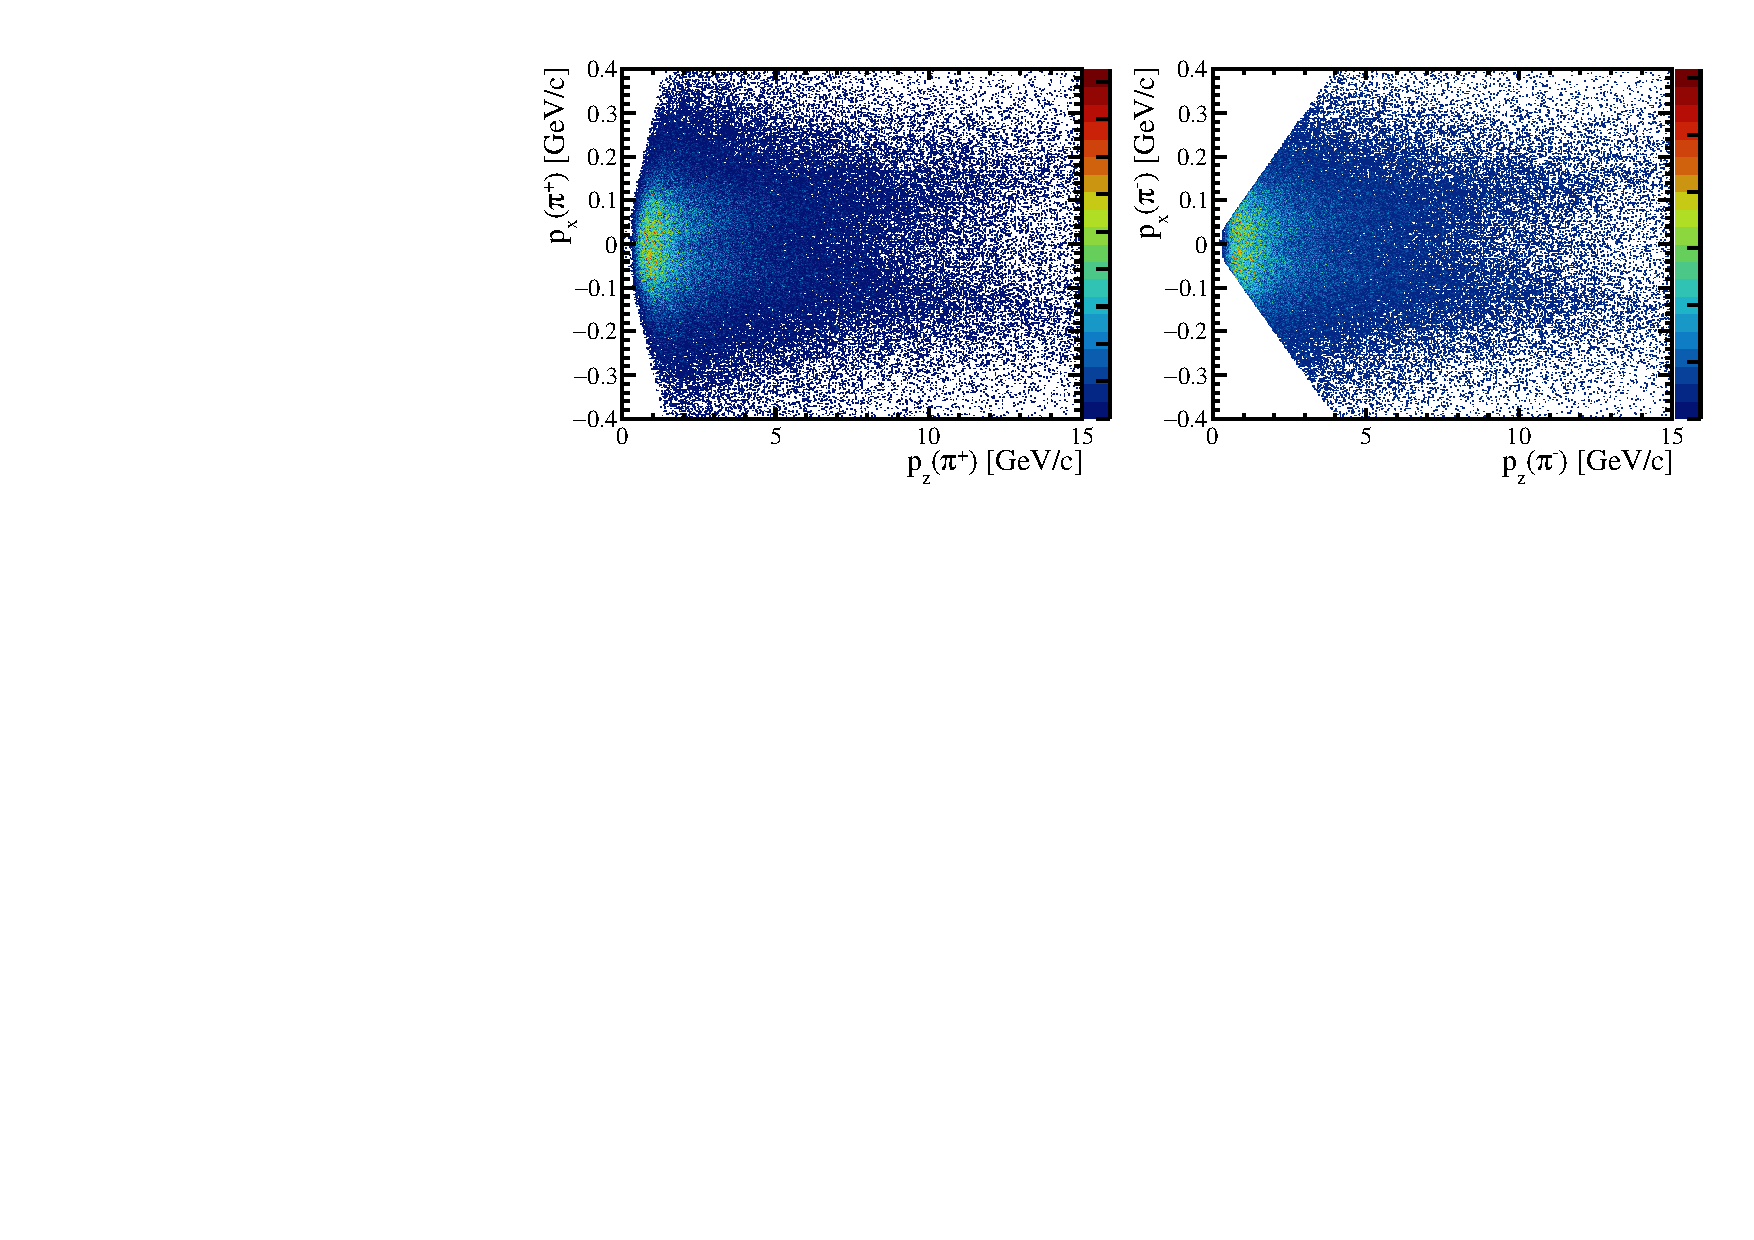
\includegraphics[width = \textwidth]{../../work/RapidSimAnalysis/MomentumDependence/Plots/sPi_C_KmKpPositiveNegative.pdf}}
        \hfill
        \subfloat{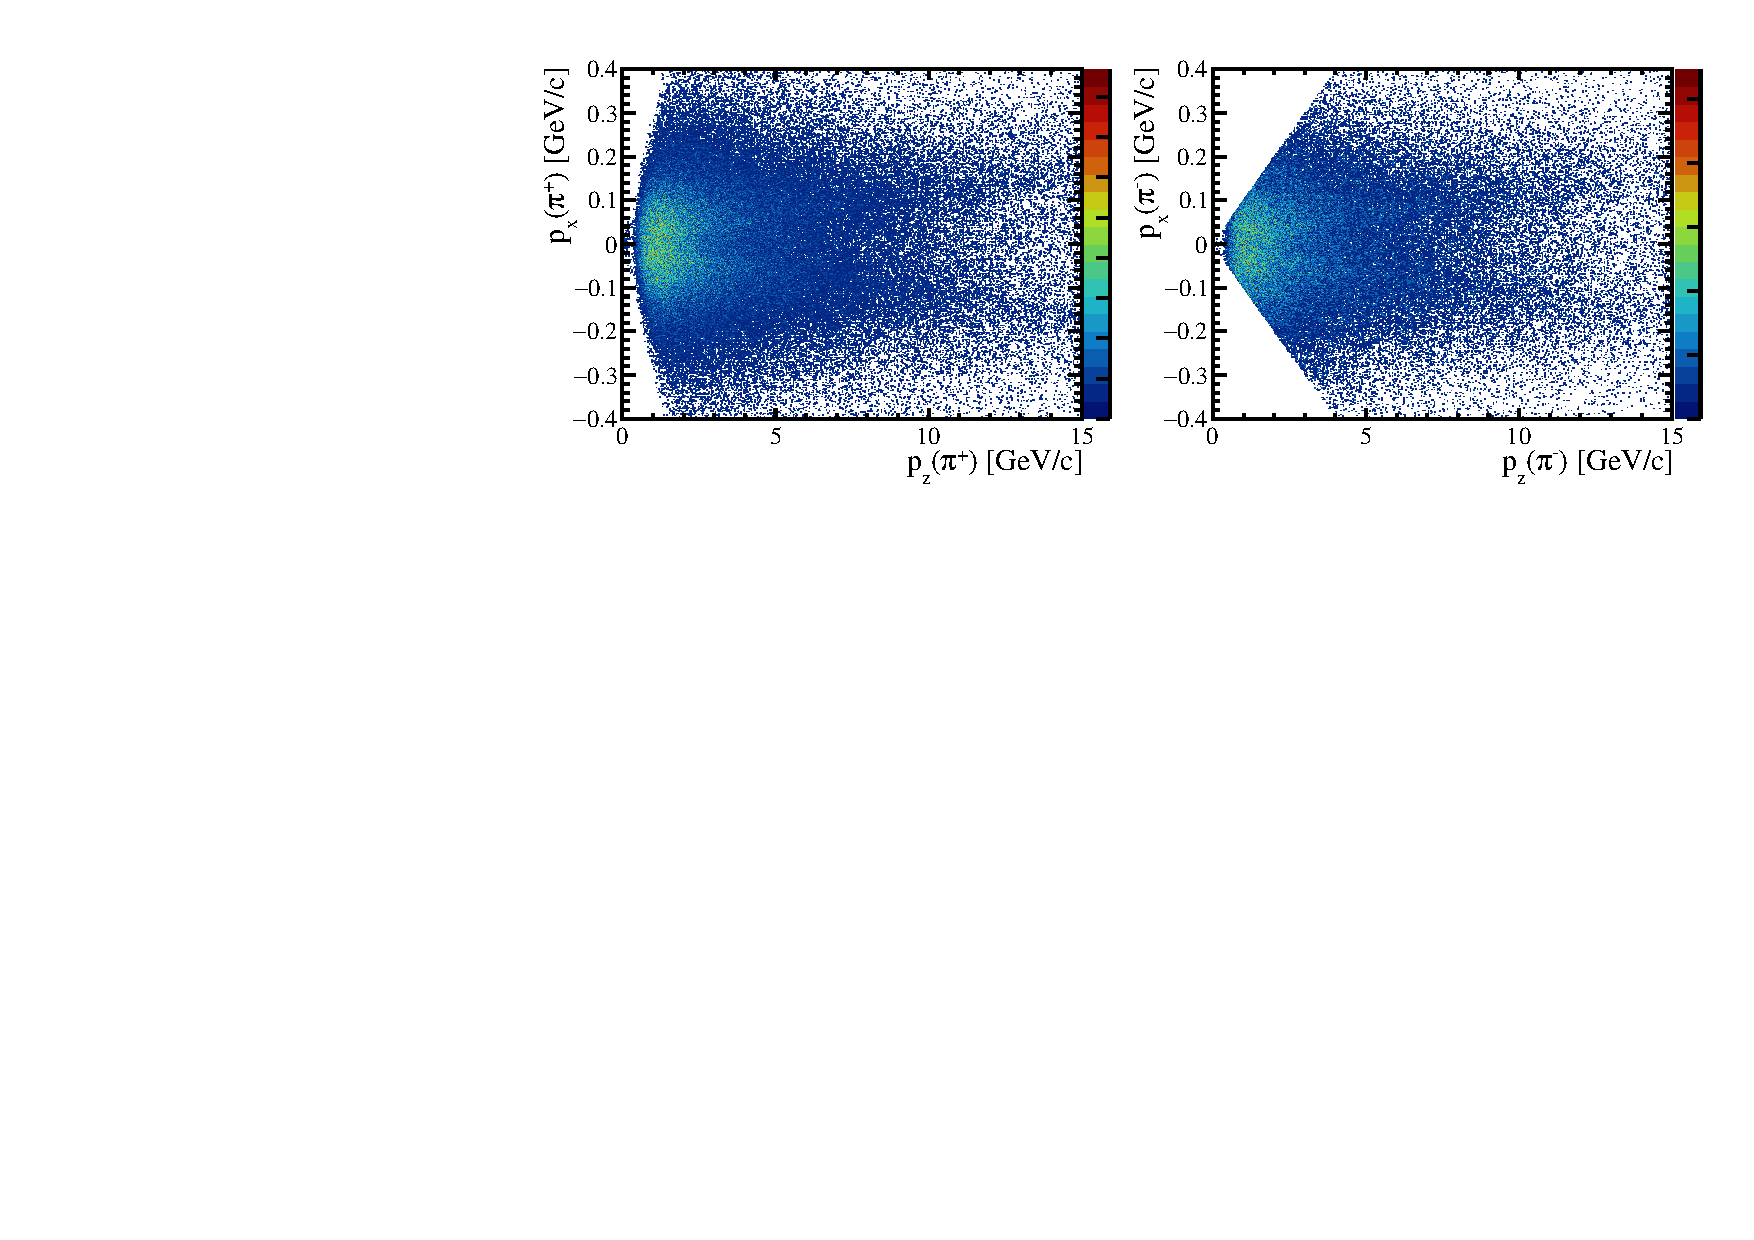
\includegraphics[width = \textwidth]{../../work/RapidSimAnalysis/MomentumDependence/Plots/sPi_C_pimpipPositiveNegative.pdf}}
        \caption{Soft $\pi$ $p_x - p_z$ plane for $D^{0}\to K^-K^+$(top) and $D^{0}\to \pi^-\pi^+$(bottom) for $\pi^+$ and $\pi^-$ after inrtoducing detection asymmetry.}
    \end{figure}

    In order to acquire the \textit{ integrated detection asymmetry} we have to perform the following integrals
    \begin{equation}
        A_D = \frac{\int \dd \vec{p}N(\vec{p})A_D(\vec{p})}{\int \dd \vec{p}N(\vec{p})}
    \end{equation}
    where each integral is accompanied with an error $\sqrt{N}$ where $N$ is the total number of entries used for the calculation.

    The total asymmetry can be measured using
    \begin{equation}
        A_{\text{total}} = \frac{N^+ - N^-}{N^+ + N^-}
    \end{equation}
    and the error can be estimated using the standard error propagation
    \begin{equation}
        \sigma A_{\text{total}} ^2 = \left(\pdv{A_{\text{total}}}{N^+}\sigma N^+\right)^2 + \left(\pdv{A_{\text{total}}}{N^-}\sigma N^-\right)^2
    \end{equation}

    However, we can use 
    \begin{equation}
        A_{\text{total}} = \frac{A_{CP} + A_D}{1 + A_{CP}A_D}
    \end{equation}
    to estimate the expected total asymmetry, where $A_{D}$ is the integrated detection asymmetry.

    We present the asymmetry results for both decays in the following tables:
    \begin{center}
        \begin{tabular}{c|c|c}
            Asymmetry & Expected & Calculated\\
            \hline\hline
            $A_{CP}$ & 0.1 & $0.0998\pm0.0012$\\
            $A_{D}$ & - & $0.0688\pm0.0016$\\
            $A_{\text{total}}$ & $0.1677\pm0.0016$ & $0.1621 +/- 0.0014$\\
        \end{tabular}
        \captionof{table}{Asymmetries for $D^0\to K^-K^+$ TTree.}
    \end{center}

    \begin{center}
        \begin{tabular}{c|c|c}
            Asymmetry & Expected & Calculated\\
            \hline\hline
            $A_{CP}$ & 0.2 & $0.2005\pm0.0016$\\
            $A_{D}$ & - & $0.0561\pm0.0018$\\
            $A_{\text{total}}$ & $0.2533\pm0.0017$ & $0.2453\pm0.0017$\\
        \end{tabular}
        \captionof{table}{Asymmetries for $D^0\to pi^-\pi^+$ TTree.}
    \end{center}
    
\end{document}